\documentclass[journal]{IEEEtran}
\usepackage{epsf,cite,amsmath,amscd,graphics,graphicx,latexsym,multicol,setspace}
\usepackage{amsfonts,amsmath,amssymb,amsthm}
\usepackage{multirow}
\usepackage{scalefnt}
\usepackage{subfigure}
\usepackage{array}
\newcounter{MYtempeqncnt}
\begin{document}
\title{Racing with Deep Reinforcement Learning}
\author{Walter A. Freire, Kevin M. Freire\\
andrei.freire@ryerson.ca, kfreirea@ryerson.ca\\
Ryerson University, Toronto, Canada.}
\maketitle

\begin{abstract}
Self driving vehicles have increased in popularity over the recent years and much research has been done in improving autonomous vehicles.  In this project we will be focusing on self driving race cars, using AWS' resources and observe the effects of training models using a deep architecture and comparing it to a shallow architecture.  We will also look into the effects of tuning hyper parameters and the effect they have on training deep Reinforcement Learning models.  This report shows the effect that a deep network have on training an agent to complete a track as fast as possible.
\end{abstract}

\section{Introduction}
Reinforcement Learning (RL) has been used to accomplish various robotic tasks such as manipulation, navigation, flight, interaction, motion planning and many more. When implementing an RL model into the real world, due to its high sample complexity, safety requirements and cost it is common to train the RL agent in a simulation. In Autonomous driving, RL require many disciplines and equipment such as access to a physical robot/car with proper sensors, an accurate robot model for simulation to avoid damaging expensive hardware in initial development, a diverse training mechanism and custom modification of the training procedure such as modifying the neural network architecture and the loss function \cite{9197465}. For our experiment we used DeepRacer as a guideline to implement and modify an existing Jupyter notebook using AWS Sagemaker and Robomaker APIs.

We decided to get started with DeepRacer because it supports state-of-the-art deep RL algorithms \cite{caspi10reinforcement}, simulations with OpenAI Gym interface \cite{brockman2016openai}, distributed rollouts and integration with cloud services. DeepRacer uses a 1/18th scale car of a physical robot that uses RL for navigation of a race track with a fish-eye lens camera \cite{9197465} with other specs such as GPU, live streaming view and more. In this paper the robot model in DeepRacers simulation is used along with the multiple provided race tracks. With the provided sources the RL model policy is trained with different simulation parameters and multiple tracks in parallel using distributed rollouts.

DeepRacer is a great platform for learning an end-to-end policy for navigating through a race track, that uses a single gray scale camera image as observation and discretized throttle/steering ad actions. The training is done in simulation using Proximal Policy Optimization (PPO) algorithm \cite{schulman2017proximal}, which can converge in under 5 minutes and about 5000 simulation steps. DeepRacer provides an interactive experience in training a vehicle to drive itself through a race track with minimal supervision. We were mainly interested in the available jail-broken version in order to modify their source code to implement our own network architecture, customize the action-space, the reward functions and much more.  This is because DeepRacer was very limited to what we can do and were restricted to their built in architectures. For this paper we implemented a simulation using AWS Robomaker and Training Deep reinforcement algorithm using the Sagemaker API to build a custom deep architecture and custom reward function in a built simulation environment built by AWS.  

The purpose of selecting this project was to learn and understand the effect of training a vehicle with RL using deep neural networks with large datasets of videos that require high computational power using the Clipped PPO algorithm and customized reward function.  \cite{7830823} States that deeper networks reduce training time in self driving vehicles.  This is an observation we will attempt to capture in our project.  The rest of the report consists of the problem statement along with the environment we used, the custom deep architecture, the reward function, the reinforcement algorithm, experiment setup , results, and discussion of results.  The full implementation will be available on Github \footnote{ Code available at https://github.com/wfrei020/DeepRacer-Freire}.

\section{Problem Statement and Environment/Dataset}
The main objective of this problem is autonomous racing.  This problem requires the agent (car) to stay in the track and drive itself while completing the track as fast as possible.  This problem is divided into separate sections which include:

\begin{enumerate}
  \item Develop the deep neural network architecture
  \item Creating the simulation environment.
  \item Create the reward function and action space.
  \item Create the proper hyper parameters for training.
  \item Collect results, test and compare to AWS shallow network.
\end{enumerate}

To develop a neural network we realize that there are many implementations to this but we decided that we wanted to learn and observe the effects of a deep neural architecture consisting of 8 convolutional layers and 2 dense layers with each layer going through a ReLU activation function.  To create our simulation environment we used AWS Sagemaker and Robomaker along with a AWS Simulation package to have a simulation environment out of the box which made this project possible in the short time frame.  AWS provided us with a simulation environment of many racetracks.  We decided to perform our experiment on the racetrack as seen in Figure \ref{reinvent}.

\begin{figure}[htbp]
\begin{center}
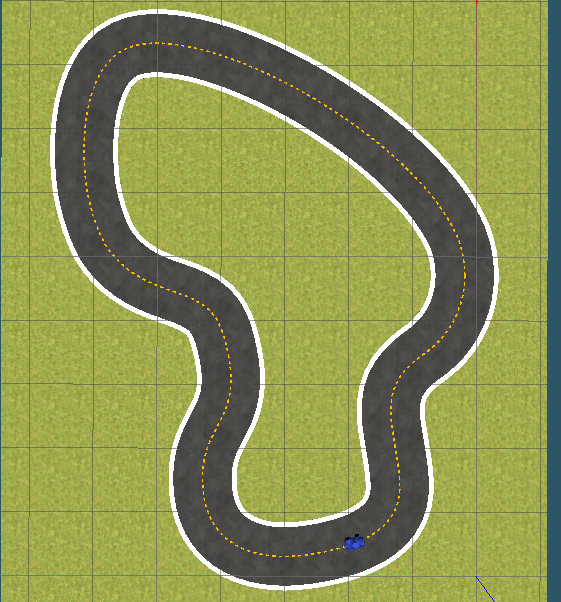
\includegraphics[width=8cm]{training_track}
\end{center}
\vspace{-2mm}
\caption{A Simplified Environment}
\label{reinvent}
\end{figure}

In order to train our agents one of the most important steps was our reward function and action space.  Our action space was a steering angle and speed of the agents.  Specifically the steering angle was from a range between -30 $^{\circ}$ to +30 $^{\circ}$ and the speed from 0.5 to 2 \emph{m/s}, along with a front facing camera as it's sensor.  We did this for a continuous action space to implement and train using the Clipped PPO algorithm.  Finally our rewards function was very complex as we returned specific rewards depending on the state of the agent.  For example, if the agent would have half a wheel off track it would return a negative reward, or if the steering angle was not correct it would return a negative reward.  If the agent had desirable actions at a specific state we would return a positive reward.  The parameters we worked with for the reward function are:

\begin{enumerate}
  \item Flag to indicate if the agent is on the track
  \item Distance in meters from the track center
  \item Flag to indicate whether the agent has crashed.
  \item Percentage of track completed
  \item Flag to indicate whether the agent has gone off track.
  \item The width of the track
  \item The agents’ speed in meters per second (m/s)
  \item The number steps completed
  \item The agents’ steering angle in degrees
  \item Flag to determine if an agent is left of the center line
\end{enumerate}

The track defines where the agent can go and what state it can be in, thus explores the environment to collect data in order to train the neural network. The agent's data is a single grayscale monocular image captured by the front-facing camera as input which represents the agent's current state. Depending on the current state an action from the agent corresponds to a move at a particular speed and steering angle. The reward is the score given as feedback to the agent when the action at a given state is taken.  The reward is returned by a reward function where you can define a reward function to specify what is a desirable or undesirable action.

In the simulator the agent explores the environment and builds up experience, the experiences collected are used to update the neural network periodically and the updated model is used to generate more experiences.   A simplified example of the environment is shown in Figure \ref{simplifiedTrack}.  By observing Figure \ref{simplifiedTrack}, each state represents an individual state. The vehicle is allowed to move up or down while facing in the direction (left to right). In order to achieve the shortest path it must follow a straight line, thus achieving the highest possible reward.  However, if the vehicle steers off track it will not receive any reward or would receive a negative reward (depending on reward function).

\begin{figure}[htbp]
\begin{center}
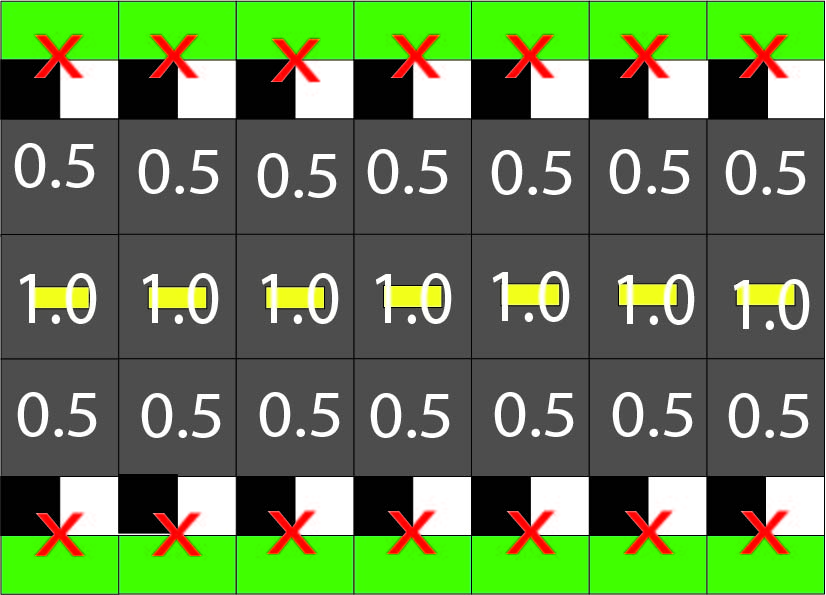
\includegraphics[width=8cm]{AWS-simplifiedTrack}
\end{center}
\vspace{-2mm}
\caption{A Simplified Environment}
\label{simplifiedTrack}
\end{figure}

The next part was to identify the proper hyper parameters.  We felt it was easier to keep some default hyper parameters since we implemented our own architecture and reward functions and we did not want to fine tune the models as much because training would cost us a lot of money and doing a fine tuning test would be too costly for this project.  
Finally in the last section we needed to record the correct results and since this was a race, we looked at time completion and how many times the agent went off track during the test.  For the training however we collected the reward it obtained during each episode.

\section{Methods and Model}
\subsection{The Architecture}
To implement our architecture we chose to go with a really deep implementation which consists of 8 convolutional layers and 2 dense layers with ReLU activation functions after each layer. The architecture is shown in Figure \ref{freire_arch}, for the convolutional design we picked these many layers mainly for educational purposes to observe the results in having this many convolutional layers.  For our final test we will be running a shallow network to see how it compares to our deep architecture.  The shallow network architecture provided by AWS is shown in the appendix.  Finally the Dense layers have a dropout rate of 50\% to handle overfitting.  This way the deep architecture does not overfit on one race track and we can see how it trains on other tracks.

\begin{figure*}[t]
\begin{center}
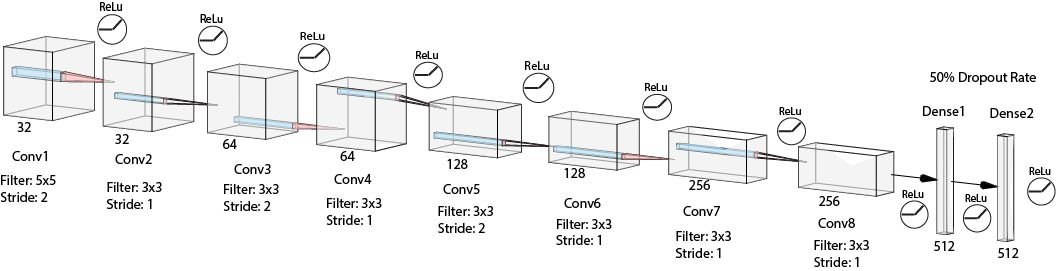
\includegraphics[width=\textwidth]{freire-arch}
\end{center}
\vspace{-2mm}
\caption{A Simplified Environment}
\label{freire_arch}
\end{figure*}

\subsection{Action Space}
As mentioned above we used an action space such that the agents can perform an action that consists of a steering angle and a speed.  Since this is a continuous action space we have many possibilities.  The actions that the agent can take is between -30 $^{\circ}$ to +30 $^{\circ}$ and between 0.5 to 2 \emph{m/s}. 

The angles were chosen based on the maximum limits that amazon provides, the speed we specifically chose to be 2 \emph{m/s} to be our max instead of 4 \emph{m/s} because we noticed that starting of training at really fast speeds can delay the training a lot, specifically when we are just starting to train.  A question that arises is whether we can slowly transfer and learn from models that were trained at slower speed and fine tune it changing the action space and train it at higher speeds. 

\begin{figure}[htbp]
\begin{center}
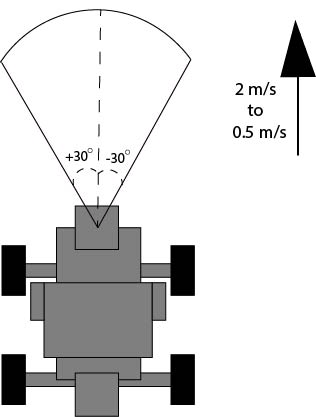
\includegraphics[width=8cm]{model-S}
\end{center}
\vspace{-2mm}
\caption{Simplified car model with max steering angles and speed range}
\label{car}
\end{figure}

\subsection{Reward Function}
The reward function that we used for all the tests are based on several considerations that affect the returned reward.  The reward function that we used is in the README file and below is a summary of how we implemented it to train our agent:

\begin{enumerate}
  \item If crashed or off track return -1 reward (handles terminal state)
  \item If car is on the left lane and all the wheels are not on the track and steering angle is to the left return -1 reward (handles terminal state because the next action will be terminal state since it will drive off track)
  \item If car is on the right lane and all the wheels are not on the track and steering angle is to the right return -1 reward (handles terminal state because the next action is terminal state since it will drive off track)
  \item Handle the opposite reward for steps b and c, return a reward based on the steering handle that return them back to the track (handles desirable action)
  \item If no wheels are off track and agents are in a desirable state return a +1 reward and if the speed is fast proportionally add to reward. (handles desirable state)
  \item Finally return  a reward of +10 if the agent finished the track in 100 steps or less (handles a positive terminal state)
\end{enumerate}

\subsection{Reinforcement Algorithm}
Proximal Policy optimization (PPO) is currently a standard use in self driving vehicles.  AWS provided two algorithms: the Soft Actor Critic (SAC) algorithm and Clipped PPO algorithm.  We decided to go with CPPO because we wanted to use an algorithm that's popular in self driving vehicles, and for its on-policy learning algorithm which is done by PPO.  On-policy algorithms tend to be more stable and exploit exploration which is why we decided to train it using the Clipped PPO algorithm.  We did not do any modification to the algorithm but rather just used the API which was implemented by Intel RL Coach framework used within AWS Sagemaker.

\subsection{Hyperparameters}
As mentioned above we did not want to focus on fine tuning the model because it was too costly using AWS resources. We focus on two sets of hyper parameters for our tests in order to observe which is better.  Shown in Table \ref{hyper-parameters} are the hyper parameters used for the experiments.

\begin{table}
\centering
\caption{Hyperparameters used for training}
\begin{tabular}{ | m{4cm} | m{4em}| m{4em} | } 
\hline
\textbf{CPPO Hyper Parameters} & \textbf{Set 1} & \textbf{Set 2} \\ 
\hline
Batch size & 64 & 64 \\ 
\hline
Epochs & 10 & 15 \\ 
\hline
Learning rate & 0.0003 & 0.0025 \\ 
\hline
Exploring type & Categorical & Categorical \\ 
\hline
$\epsilon$-greedy & 1 & 0.9 \\ 
\hline
Beta entropy & 0.01 & 0.01 \\ 
\hline
Discount factor & 0.95 & 0.95 \\ 
\hline
Loss type & Huber & Huber \\ 
\hline
\# of episode between training & 20 & 20 \\ 
\hline
\end{tabular}
\label{Hyperparameters}
\end{table}

\subsection{Testing Metrics}
Finally for the training metrics we wanted to observe some important information.  Since this is a race we observed 3 metrics.  The first was the completion of the track, this was important because it must complete the track fully to finish the race.  Second we wanted to record how often the agent went off track and finally the most important result is to see how fast the agent completed the track.  Track completion, off track count and time to complete the track were the metrics we used to compare the models we trained.

\subsection{Model Comparison}
Since we wanted to test the effect of training a deep network using reinforcement learning we needed to test and compare against another architecture.  AWS provided a built in architecture which we used to start our test that used a shallow architecture which only consists of 3 convolutional layers and no dense layers. The convolutional layers had a design where the first layer has 32 filters using 8$\times$8 filter and stride of 4 followed by a ReLU activation function.  The second layer has 64 filters using 4$\times$4 filter and stride 2 followed by a ReLU function and finally the third layer has 64 filters using 3$\times$3 filter and stride of 1.  We ran the same test we ran in our architecture in order to compare results fairly.  As mentioned earlier, the object is to observe if a deeper network can reduce training time in self driving vehicles.

\section{Results and Discussion}
For our initial set of results we wanted to test the effect of using different hyper parameters, so we trained it using two sets of hyper parameters as shown in Table \ref{twoHyperSets}.  In our case set 1 did better with a faster time and less times off track using both the architectures.  So for the rest of the tests we decided to use the set 1 hyper parameters.

\begin{table}
\centering
\caption{Training using two sets of hyperparameters}
\begin{tabular}{ |p{3cm}|p{1cm}|p{1cm}|p{1cm}|p{1cm}|  }
\hline
\multirow{2}{4em}{Hyperparameter Set} & \multicolumn{2}{|c|}{Deep Network} & \multicolumn{2}{|c|}{Shallow Network} \\
\cline{2-5}
 & Time & Off Track & Time & Off Track \\
\hline
1 & 15.034 & 3  & 15.255 & 0 \\
\hline
 2 & 16.952 & 8  & 17.207 & 10 \\
\hline
\end{tabular}
\label{twoHyperSets}
\end{table}

Our main goal for this project was to identify the effect of training a self driving vehicle using a deep architecture that we implemented and compare it to a shallow architecture provided by AWS.  As shown in Table \ref{mainTest} we performed the 3 training jobs and each architecture was trained for 1 , 4, and 8 hours. 

\begin{table}[t]
\centering
\caption{Training comparison}
\begin{tabular}{ |p{1cm}|p{2cm}|p{1cm}|p{2cm}|p{1cm}| }
\hline
 \multirow{2}{*}{Hours} & \multicolumn{2}{|c|}{Deep Network} & \multicolumn{2}{|c|}{Shallow Network} \\
\cline{2-5}
 & Elapse Time (s) & Off Track &  Elapse Time (s) & Off Track  \\
\hline
\multirow{1}{4em}{1} & 55.382 & 2 & 21.245 & 0 \\ 
 \hline
\multirow{1}{4em}{4} & 15.034& 3 & 15.255 & 0 \\ 
 \hline
\multirow{1}{4em}{8} & 14.385& 2 & 13.545 & 0 \\ 
 \hline
\end{tabular}
\label{mainTest}
\end{table}

Looking at the results you can see that the 1 hour test for both cases took a long time to complete the track.  Our deep network took 50+ seconds to complete it while the shallow network only took 20+ seconds.  It is clear to see that when you only train for 1 hour a shallow network performs better.  So we proceeded to experiment again for 4 hours and observed that our initial objective was starting to show.  The deep and the shallow network have around the same time to complete the track.  This test demonstrates that in 4 hours a deeper network was able to achieve the same results as shallow.  The deeper network improved by 73\% with an additional 3 hours of training while the shallow network only improved by 28\%.  

[need to add final results here]

Looking at the results in Table \label{mainTest} we see that the deeper network tends to train faster and improve overall results of a self driving race car.  This has some conditions as you can see because a deep network does not perform as well with only 1 hour of training like the shallow architecture did.  As soon as the training time surpassed 4 hours of training that's when we saw that the deep architecture started surpassing performance of shallow networks.  Unfortunately from our result we saw that after 8 hours of training the shallow network did better on average by 0.84 seconds.  This brings up a lot of questions on why this deep network did not perform better than the shallow network.  It could be that the PPO algorithm does not require deep networks in tasks that involve speed.  Speed in this task is an essential component and if an agent needs a lot of time to make a decision due to its processing then a deep network may not have been the solution.  This is something we did not consider when we were implementing a self driving race car.  The processing time for each state may have affected the overall time it took to complete a racetrack.  A deeper network has more hidden states that it must process at every state, compared to a shallow network.  We understand now that deeper networks need more time to process more data and these task must not rely on speed to complete, it may be better to use shallow network, when it comes to tasks that involve quick decisions.

As a final test we wanted to see the models trained on different tracks and observe their results.  We trained for 8 hours on the reinvent track and test it on two other tracks as shown in the Appendix.  You can see that our deep architecture did not do as good as the shallow network.  Not only that but the agents went off track more in the deeper network.  As mentioned above this could be due to the fact that the deeper network needs longer processing time to make a decision which is a disadvantage in a speed task.

\begin{table}[t]
\centering
\caption{Testing comparison Different Tracks}
\begin{tabular}{ |p{2cm}|p{1.25cm}|p{1cm}|p{1.25cm}|p{1cm}| }
\hline
 \multirow{2}{4em}{Track} & \multicolumn{2}{|c|}{Deep Network} & \multicolumn{2}{|c|}{Shallow Network} \\
\cline{2-5}
 & Elapse Time (s) & Off Track &  Elapse Time (s) & Off Track  \\
\hline
Reinvent (trained) & 14.385	 & 2 & 13.545	 & 0 \\ 
 \hline
Monaco (Complex) & 47.283	 & 18 & 45.022	& 19 \\ 
 \hline
Oval (Simple) & 14.233	 & 7 & 13.71 & 5 \\ 
 \hline
\end{tabular}
\label{DiffRacetrackTest}
\end{table}


This project has much research to continue on such as discovering what are the best hyper parameters for a deep network.  We also would like to identify what else is affected by deeper networks such as overfitting certain race tracks.  There are other tests we would've liked to implement such as the activation functions that we used in between all our layers.  We used ReLU but what would have happened if we used TANH or other functions?  Using deep networks is a popular solution to self driving cars but may not be a good solution for tasks that involve quick decisions.  There are so many areas to proceed in this task such as asking the question that even though a deep network did not do good in a race but how about an obstacle avoidance task?

\section{Implementation and Code}
As mentioned throughout the paper we used Amazons’s Sagemaker API and python’s python development environment.  Sagemaker Library used the RL Coach from Intel for the reinforcement learning Algorithms.  The code is available on Github along with our modification of the code we implemented.  The github repo is available at \emph{https://github.com/wfrei020/DeepRacer-Freire}, please read the README file for additional details.  For the simulation, amazon used robomaker and we implemented and ran it using a GPU.  The original notebook provided by AWS for Deepracer was outdated and we spent a lot of effort and time upgrading it to the newest version.  The notebook was available at \emph{https://github.com/aws/amazon-sagemaker-examples} and we upgraded it using the help of issue number 2055.  This helped us upgrade a lot of the packages.  Finally we also had to make the notebook compatible for CPPO.  The notebook that AWS provided only worked for the SAC algorithm.  We really wanted to work with CPPO so we spent several days debugging and adding some code fix to allow the use of CPPO.  In the Appendix we have some important code we implemented for our project but we will not be including all the fixes throughout the API as it is too much and not important to the project. Finally in general we used AWS Dockers, Robomaker, Sagemaker ML libraries, and S3 bucket for storing our models. 

\section{Conclusion}
In conclusion we have shown the effect of training a deep network for self driving race cars.  In our experiment we found out that deeper networks may have a disadvantage to race tasks or task that speed is the main condition.  We also looked at some effects of tuning hyperparameters and saw that changing them a little bit had a big effect on overall results.  We hope to continue working on this since AWS provides monthly race competition around the world to test our models and see who implements the fastest self driving race car.

\bibliography{finalreport}
\bibliographystyle{ieeetr}

\newpage

\section{Appendix}

\subsection{Testing Race Tracks}
\begin{figure}[htbp]
\begin{center}
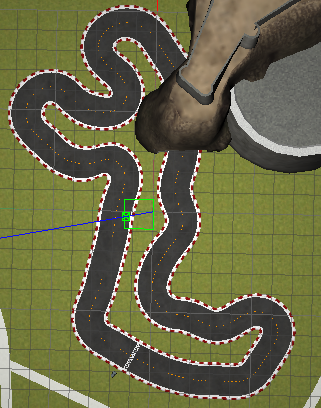
\includegraphics[width=4cm]{trainingTrack2}
\end{center}
\vspace{-2mm}
\caption{Monaco Training Track}
\label{monaco}
\end{figure}


\begin{figure}[htbp]
\begin{center}
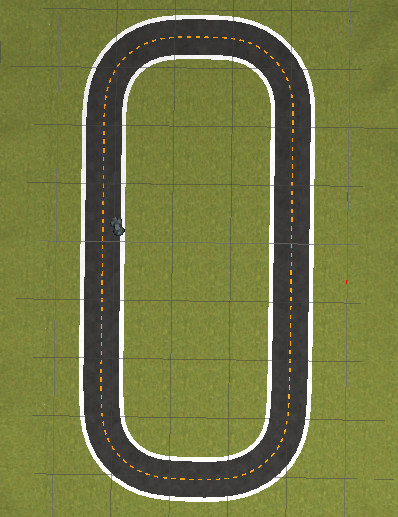
\includegraphics[width=4cm]{trainingTrack3}
\end{center}
\vspace{-2mm}
\caption{Oval Training Track}
\label{oval}
\end{figure}

\end{document}